%***********************************************************************
% PLEASE LEAVE THIS PART UNCHANGED
% No problem!
%***********************************************************************

\documentclass[twoside]{report}
\usepackage{iwsm}
\usepackage{graphicx}
\usepackage{amsmath, amssymb}
\usepackage{booktabs}

\begin{document}

%***********************************************************************
% PLEASE INSERT YOUR CONTENT FROM HERE
%***********************************************************************

% Title and running title to be used as left header:
\title{Graphical Assessment of Probabilistic Precipitation Forecasts}
\titlerunning{Graphical Assessment of Probabilistic Forecasts}
%\title{Probabilistic Precipitation Forecasts: Model comparison and Graphical Assessment}
%\titlerunning{Probabilistic Precipitation Forecast Assessment}

% Authors and running list of authors to be used as right header:
\author{Reto Stauffer\inst{1}\,\inst{2}, Moritz N. Lang\inst{1}, Achim Zeileis\inst{1}}
\authorrunning{Stauffer et\,al.}

% Institutes of all authors
% Include city and country of each institute, do not include the full address.
\institute{Department of Statistics, Universit\"at Innsbruck, Austria
\and Digital Science Center, Universit\"at Innsbruck, Austria}

% E-mail of presenting author for correspondence
\email{Reto.Stauffer@uibk.ac.at}

% Brief abstract of the paper:
\abstract{
    Accurate and reliable probabilistic predictions have been becoming more and more
    important over the last decades and they are an essential
    tool for proper risk assessment and strategic planning.
    In order to provide full probabilistic forecasts, distributional regression
    models are frequently used.  Such models range from basic generalized
    linear models (GLM) over generalized additive models (GAM) to generalized
    additive models for locate, scale, and shape (GAMLSS) and other types of
    refined distributional regression models.

    For assessing the goodness of fit of such probabilistic regression models,
    graphical assessment techniques are an important complement to proper
    scoring rules and help to identify possible model misspecifications.
    Based on a case study of probabilistic precipitation forecasts, three
    different regression models with different sources of misspecification are
    graphically evaluated within a unified framework. By evaluating the
    marginal and probabilistic calibration of the models, the commonalities of
    the different graphs are highlighted, along with their relative strengths
    and weaknesses in revealing various sources of misfit.

}

% Keywords (at most 5):
\keywords{Graphical model assessment; Probabilistic prediction; Distributional regression; Precipitation forecasts}

% Produce the title:
\maketitle

%***********************************************************************

% Sections and subsections (do not use lower levels):

\section{Case study}

Forecasting precipitation has always been one of the essential quantities in
weather forecasting not only for the public, but for many socio-economic areas
like agriculture, power production, but also decision makers with respect risk
assessments. 
The demand of accurate predictions of the expected amount of precipitation has
increased over the past decade where severe precipitation events have
become more frequent.

Weather forecasts are typically generated by physically based numerical weather
prediction models. To account for uncertainty, multiple forecasts are created
with slightly modified conditions which build an ensemble (Gneiting et\,al.
2005). This allows to not only retrieve the expected amount of precipitation
but also information about the uncertainty of a specific forecast.
To unleash the full potential of these ensemble forecasts, statistical
post-processing is often used to correct model biases and insufficiencies in
forecast uncertainty.

Building upon the work of Messner, Mayr, and Zeileis (2010), three statistical
regression models will be fitted and compared using
graphical model assessment methods.
This allows to easily identify possible misspecifications of the different
models and to select the best fitting model among a series of possible candidates.

% assumptions and to uniformly compare
%different types of models.
%This allows to easily identify to compare the different models in terms of
%possible misspecifications.

%This is especially important when comparing the raw ensemble forecasts to
%different spatial scales, e.g., to specific locations.

%%In the recent past many different
%%statistical models have been proposed using different distributional assumptions
%%and learners. For evaluation, proper scoring rules are often used which not
%%only evaluate the expectation but the full probabilistic distribution of
%%the forecasts. To identify possible misspecifications in the model
%%assumption, graphical assessment methods are particularely advantageous
%%and will be presented in this article.

\subsection{Data}

The data used contains observed 3\,day-accumulated precipitation amounts for
Innsbruck (Austria) and the corresponding ensemble mean ($\text{ensmean}$) and
ensemble standard deviation ($\text{enssd}$) of total accumulated precipitation amounts
between $5$ and $8$ days in advance.
Following previous studies, the square root of precipitation is used which has
been shown to improve the calibration.

%In previous studies it has been shown that it is of advantage to
%model the square root of precipitation rather than precipitation itself. Thus
%all precipitation amounts are square rooted before ensemble mean and standard
%deviation are derived. Furthermore, events with no variation in the ensemble
%are omitted:

\subsection{Statistical models}

For comparison, three models are fitted. A homoscedastic Gaussian linear regression
model which does not properly account for the non-negative nature of precipitation,
and two heteroscedastic left-censored regression models --
one assuming a Gaussian and one a logistic underlying response distribution:

\begin{table}[!ht]\centering
    \begin{tabular}{lll}
         Distribution                              & Location                                         & Scale \\
        \midrule[0.09 em]
        $y_i \sim \mathcal{N}(\mu_i, \sigma)$     & $\mu_i = \beta_0 + \beta_1 \cdot \text{ensmean}$ & $\sigma = \text{sd}(\epsilon)$ \\
        $y_i \sim \mathcal{N}_0(\mu_i, \sigma_i)$ & $\mu_i = \beta_0 + \beta_1 \cdot \text{ensmean}$ & $\sigma_i = \gamma_0 + \gamma_1 \cdot \log(\text{enssd})$ \\
        $y_i \sim \mathcal{L}_0(\mu_i, \sigma_i)$ & $\mu_i = \beta_0 + \beta_1 \cdot \text{ensmean}$ & $\sigma_i = \gamma_0 + \gamma_1 \cdot \log(\text{enssd})$ \\
        \bottomrule[0.09 em]
    \end{tabular}
\end{table}


\section{Model assessment}

According to the seminal work of Gneiting, Balabdaoui, and Raftery (2007),
probabilistic forecasts aim to maximize the sharpness of the predictive
distributions subject to calibration. 
In the assessment of the goodness of fit of probabilistic predictions,
it is further distinguished between marginal and probabilistic calibration.

\subsection{Marginal calibration}


Marginal calibration is generally concerned with whether the observed
frequencies match the frequencies expected by the model.  For continuous
observations, frequencies for intervals of observations are being used, while
the expected frequencies are computed by differences between the predictive
CDFs $F(\cdot)$, evaluated at the interval breaks:


$$
\text{observed}_j = \sum_{i=1}^n \omega_i I(y_i \in (b_j, b_{j+1}]),
$$

$$
\text{expected}_j = \sum_{i=1}^n \omega_i \big[ F(b_{j+1} | \hat{\theta}_i) - F(b_{j} | \hat{\theta}_i) \big].
$$

Figure~\ref{stauffer:fig1} shows so called hanging rootograms where the
observed frequencies are hanging from the expected ones. The marginal
calibration is assessed on the observational scale, which allows a direct
interpretation.  The heteroscedastic Gaussian model clearly underfits zero
precipitation amounts as it is not accounting for the observed point mass at
zero. Additionally, a weak wavelike pattern indicates a slight overfitting of
precipitation sums between $0$ and $5$ and an underfitting of precipitation
above. In contrast, the heteroscedastic left-censored Gaussian model provides a
fairly good marginal fit.

However, due to the aggregation over all predictive distributions, a statement
about a possible violation of the distributional assumption is not possible.

\begin{figure}[!ht]\centering
    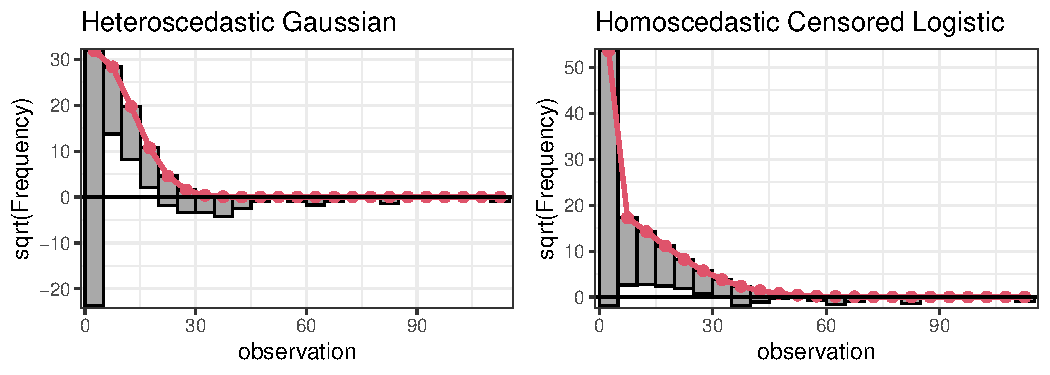
\includegraphics[width=\textwidth]{Stauffer-rootograms}
    \caption{\label{stauffer:fig1}
        Hanging rootogram for the homoscedastic Gaussian model (left)
        and the heteroscedastic left-censored Gaussian model (right).
        Expected frequencies shown in red (line), observed frequencies
        in gray (bars).
    }
\end{figure}


%Advantage: Scale of observations is natural, direct interpretation.
%Disadvantage: Needs to be compared with a combination of distributions.


\subsection{Probabilistic calibration}

Compared to the marginal calibration which is obtained on the observation
scale, the probabilistic calibration is always performed on the probability
scale. Probabilistic calibration is usually assessed using probability
integral transform (PIT) values ($u_i$) which can be mapped to other
distributional scales such as the standard Normal distribution as follows:

$$
r_i = \Phi^{-1}\big(u_i)~~\text{with}~~u_i = \begin{cases}
    F(y_i | \hat{\theta}_i) & \text{if}~F(\cdot)~\text{continuous}  \\
    U\big[F(y_i - 1 | \hat{\theta}_i), F(y_i | \hat{\theta}_i)\big] & \text{if}~F(\cdot)~\text{discrete}
\end{cases}
$$

These are also known as (randomized) quantile residuals ($r_i$; Dunn and Smyth
1996) and can be compared to the theoretical quantiles of the standard Normal
distribution.  As in Q-Q plots, small too medium deviations can be quite hard
to detect, detrending the plot by subtracting the theoretical quantiles can
make the detection of deviations from a now horizontal line easier and leads to
the worm plot.

\begin{figure}[!ht]\centering
    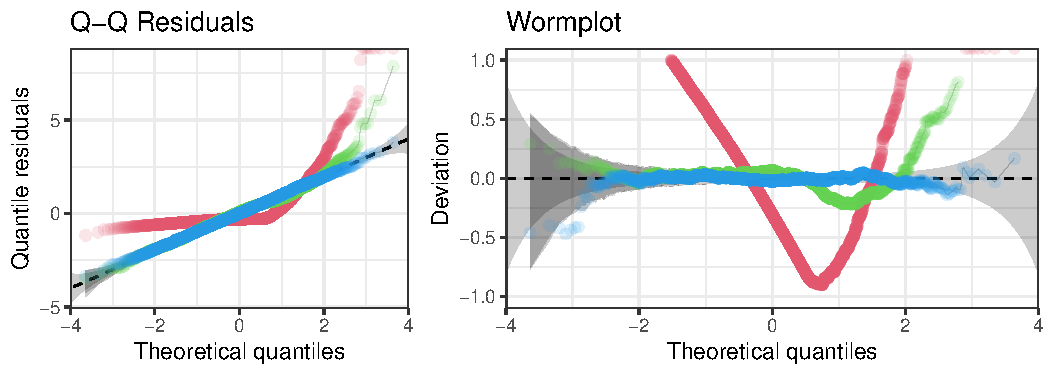
\includegraphics[width=\textwidth]{Stauffer-qqresiduals}
    \caption{\label{stauffer:fig2} 
        Q-Q plot (left) and worm plot (right) for the homoscedastic
        Gaussian model (red), as well as the heteroscedastic left-censored
        Gaussian (green) and the heteroscedastic left-censored logistic (blue) model.
    }
\end{figure}


Both, the Q-Q plot and the worm plot (Fig.\,\ref{stauffer:fig2}) show an
obvious misfit of the homoscedastic Gaussian model on both tails of the
distribution. While the marginal calibration (Fig.\,\ref{stauffer:fig1})
clearly shows that this is mainly due to missing censoring, the probabilistic
calibration does not allow to uncover the sources causing this lack of fit.

While the scale itself not easily interpretable, the probabilistic calibration
allows to check if the distributional assumption is correct.  Comparing both
left-censored heteroscedastic models, a slight advantage can be seen for the
one using a left-censored logistic distribution as its heavier tails lead to a
better fit, especially for high quantiles.

%Advantage: Needs to be compared with only one distribution (uniform or normal).
%Disadvantage: Scale is not so natural. May require randomization for discrete distributions.



%Vergleich:
%
%* Binning in marginal 'maskiert'
%* QQ/worm: pairwise; dist


%***********************************************************************

% References should be placed in the text in author (year) form.
% The list of references should be placed below IN ALPHABETICAL ORDER.
% (Please follow the format of the examples very tightly).




\references
\begin{description}
% QQ REsiduals
    \item [Dunn, P.K., and Smyth G.K.] (1996).
        Randomized Quantile Residuals.
        {\it Journal of Computational and Graphical Statistics},
        {\bf 5}(3), 236\,--\,244.
% Reliability diagram
%\item [Bröcker, J., and Smith, L.A.] (2007).
%    Increasing the Reliability of Reliability Diagrams.
%    {\it Weather and Forecasting},
%    {\bf 22}(3), 651\,--\,61.
% Ensemble forecasting
%\item[Gneiting, T., and Raftery, A.E.] (2005).
%    Weather Forecasting with Ensemble Methods.
%    {\it Science},
%    {\bf 310}(5746), 248\,--\,249.
% Proper scoring rules (CRPS)
%\item[Gneiting, T., and Raftery, A.E.] (2007).
%    Strictly Proper Scoring Rules, Prediction, and Estimation.
%    {\it ournal of the American Statistical Association},
%    {\bf 102}(477), 359\,--\,78.
% Maximize sharpness subject to calibration
\item[Gneiting, T., Balabdaoui, F., and Raftery, A.E.] (2007).
    Probabilistic Forecasts, Calibration and Sharpness.
    {\it Journal of the Royal Statistical Society: Series B (Methodological)},
    {\bf 69}(2), 243\,--\,68.
% Rootograms (marginal calibration)
%\item [Kleiber, C., and Zeileis A.] (2016).
%    Visualizing Count Data Regressions Using Rootograms.
%    {\it The American Statistician},
%    {\bf 70}(3), 296\,--\,303.
% Rain stuff 
\item [Messner, J.W., Mayr, G.J., and Zeileis A.] (2016).
    Heteroscedastic Censored and Truncated Regression with crch.
    {\it The R Journal},
    {\bf 8}(1), 173\,--\,181.
% PIT residuals (specifically)
%\item [Warton, D.I., Thibaut, L., and Wang, Y.A.] (2017).
%    The Pit-Trap---{A} ``Model-Free'' Bootstrap Procedure for Inference About
%    Regression Models with Discrete, Multivariate Responses.
%    {\it PLOS ONE},
%    {\bf 12}(7), 1\,--\,18.
% Reliability diagram
%\item [Wilks, D.] (2011).
%    {\it Statistical Methods in the Atmospheric Sciences 3rd ed}.
%    Academic Press.
\end{description}

\end{document}
